%SourceDoc ws-skript.tex
%
% c04-verteilung.tex
%
% (c) 2006 Prof. Dr. Andreas M�ller
% $Id: c04-verteilung.tex,v 1.19 2008/09/09 14:22:16 afm Exp $
%
\rhead{Verteilung}
\chapter{Wahrscheinlichkeitsverteilung\label{chapter-wahrscheinlichkeitsverteilung}}
Mit dem Begriff der Ereignisalgebra kann man nur dann Wahrscheinlichkeiten
und Erwartungswerte einfach berechnen, wenn nur endlich viele 
Elementarereignisse "uberhaupt vorkommen. Schon das Beispiel der
Messungen auf der reellen Achse hat gezeigt, dass man mit diesem
Begriff zwar sch"one Ereignis-Diagramme zeichnen kann, aber die Berechnung
zum Beispiel von Wahrscheinlichkeiten schwierig wird.

\section{Wahrscheinlichkeitsverteilung}
\begin{figure}
\begin{center}
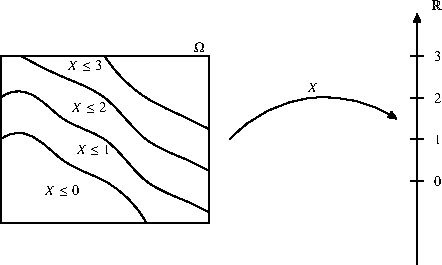
\includegraphics[width=0.9\hsize]{images/verteilungsfunktion-1}
\end{center}
\caption{"Ubergang von der Ereignisalgebra $(\Omega,{\cal A})$ zu Werten
der Zufallsvariablen $X$\label{bilduebergangzurverteilungsfunktion}}
\end{figure}
In diesem Abschnitt suchen wir daher nach einer Methode, mit der
man zuf"allige Ereignisse besser in den Griff bekommen kann, wenn
damit reelle Werte verbunden sind. Es geht also um Situationen, wo
man neben der Ereignisalgebra $(\Omega,{\cal A})$ auch noch eine
Zufallsvariable $X\colon \Omega\to\mathbb{R}$ hat. 

\subsection{Verteilungsfunktion}
\index{Verteilungsfunktion}
\begin{figure}
\begin{center}
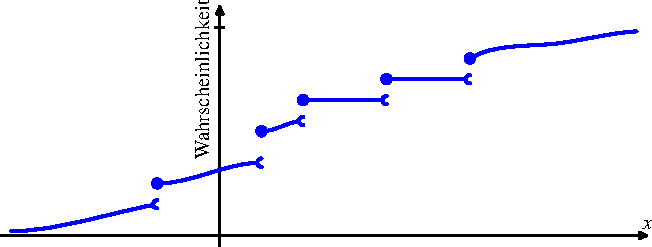
\includegraphics{images/verteilungsfunktion-2}
\end{center}
\caption{Die Verteilungsfunktion $F$ einer Zufallsvariablen $X$,
$F(x)=P(X\le x)$, zeigt die Wahrscheinlichkeit daf"ur, dass $X$ den Wert $x$ nicht "uberschreitet\label{bildverteilungsfunktion}}
\end{figure}
Aus einem Wahrscheinlichkeitsmass $P$ auf $\Omega$ kann man mit Hilfe
von $X$ auch ein Wahrscheinlichkeitsmass auf $\mathbb{R}$ bilden. F"ur die
Wahrscheinlichkeit f"ur das Interval $[a,b]\subset\mathbb{R}$ setzt
man einfach
\[
P((a,b])=P(a< X\le b)=P(X^{-1}((a,b])),
\]
das letzte $P$ ist dabei als Wahrscheinlichkeit eines Ereignisses $\Omega$
bereits bekannt.
Noch etwas handlicher ist die folgende Definition

\begin{definition}
Die Funktion $F\colon\mathbb{R}\to\mathbb{R}:x\mapsto P(X\le x)$
heisst Verteilungsfunktion von $P$.
\end{definition}
Die Funktion ist immer eine monoton wachsende Funktion, denn
\[
F(b)-F(a)=P(a<X\le b)\ge 0\quad\text{falls}\quad a\le b.
\]
Die Wahrscheinlichkeit des sicheren Ereignisses ist 1, also
$\lim_{x\to\infty}F(x)=1.$
Die Verteilungsfunktion $F$ beinhaltet alle Information, um $P$ zu
rekonstruieren. Man kann mit ihrer Hilfe auch die Wahrscheinlichkeit
abgeschlossener Intervalle oder offener Intervalle berechnen:
\begin{satz} Sei $F$ die Verteilungsfunktion der Zufallsvariablen $X$,
dann gilt
\begin{eqnarray*}
P((a,b])&=&F(b)-F(a)\\
P([a,b])&=&\lim_{\xi\to a-} P((\xi,b])=F(b)-\lim_{\xi\to a-}F(\xi)\\
P((a,b))&=&\lim_{\xi\to b-} P((a,\xi])=\lim_{\xi\to b-}F(\xi)-F(a)\\
P([a,b))&=&\lim_{\eta\to b-}\lim_{\xi\to a-} P((\xi,\eta])=\lim_{\eta\to b-}F(\eta)-\lim_{\xi\to a-}F(\xi)\\
\end{eqnarray*}
\end{satz}
\begin{proof}[Beweis]Durch Nachrechnen unmittelbar aus den Definitionen.
\end{proof}
Als Spezialfall erh"alt man auch die Wahrscheinlichkeit f"ur einen einzelnen
Wert
\[
P(a)=P([a,a])=F(a)-\lim_{\xi\to a-}F(\xi).
\]
Solange die Funktion $F$ stetig ist, wird diese Wahrscheinlichkeit
verschwinden. Andernfalls hat die Verteilungsfunktion am Punkt $a$ eine
Sprungstelle, und die Wahrscheinlichkeit, dass der Wert $a$ eintritt,
ist gerade die Sprungh"ohe.

Man kann zeigen, dass eine monotone Funktion nur abz"ahlbar viele Sprungstellen
hat. Es gibt also eine Folge $(a_k)_{k\in\mathbb{N}}$, welche alle
Sprungstellen enth"alt. Diese Werte zeichnen sich dadurch aus, dass ihre
Wahrscheinlichkeit nicht $0$ ist und der Sprungh"ohe entspricht:
\[
P(a_k)=F(a_k)-\lim_{x\to a_k-}F(x).
\]
Aus diesen Sprungstellen kann man jetzt eine Funktion konstruieren,
die nur die Sprungstellen ber"ucksichtigt:
\[
F_d(x)=\sum_{k=1, a_k\le x}^\infty P(a_k)
\]
Die Funktion $F_d$ hat genau die gleichen Sprungstellen wie $F$, und
auch die gleichen Sprungh"ohen. $F_d$ kann sich nur "andern, wenn in der
Summe ein neuer Summand hinzukommt, also is $F_d$ zwischen den Sprungstellen
konstant.
\index{Sprungstelle}

\begin{figure}
\begin{center}
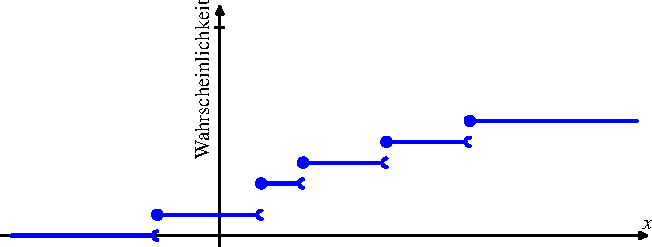
\includegraphics{images/verteilungsfunktion-3}
\[
+
\]
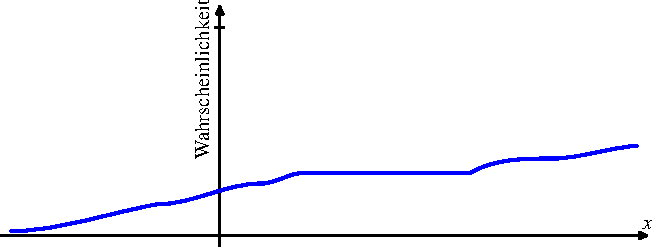
\includegraphics{images/verteilungsfunktion-4}
\[
=
\]
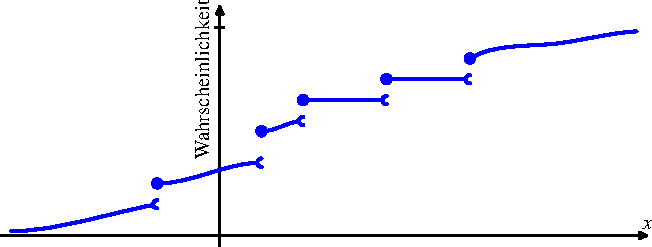
\includegraphics{images/verteilungsfunktion-2}
\end{center}
\caption{Zerlegung einer beliebigen Verteilungsfunktion (unten) in diskrete (oben)
und stetige (mitte) Komponente\label{bildzerlegungverteilungsfunktion}}
\end{figure}
\index{Verteilung!diskrete}
\index{Verteilung!stetige}

Die Differenz $F_s=F-F_d$ kann offensichtlich keine Sprungstellen haben,
wenigstens kein Sprungstellen bei Ann"aherung von links. Damit liegt
die Vermutung nahe, dass $F_s$ eine stetige Funktion ist (daher der Index
$s$). Das ist tats"achlich so:
\begin{satz}Eine Verteilungsfunktion $F$ kann immer zerlegt werden in eine
st"uckweise konstante, monoton wachsende, rechtsseitig stetige Funktion
$F_d$ und eine stetige Funktion $F_s$:
\[
F=F_d+F_s,
\]
ausserdem ist diese Zerlegung eindeutig.
\end{satz}
Die Zerlegung der Verteilungsfunktion $F$ ist in
Abbildung~\ref{bildzerlegungverteilungsfunktion} dargestellt.
\begin{proof}[Beweis]
Es gen"ugt offensichtlich zu zeigen, dass $F$ rechtsseitig stetig ist, also
keine Sprungstellen bei Ann"aherung von rechts hat. Die Differenz
$F(a+\varepsilon)-F(a)$ ist die Wahrscheinlichkeit, dass der Wert der
Zufallsvariable in das Interval $(a,a+\varepsilon]$
f"allt. Es genugt, wenn man f"ur $\varepsilon=\frac1n$ zeigen kann,
dass $F(a+\frac1n)\to F(a)$. Das Interval $(a,a\frac1n]$ kann man
als Vereinigung unendlich vieler kleiner Teilintervalle
schreiben, also
\[
\left(a,{\textstyle a+\frac1n}\right]
= \left(a,a+{\textstyle \frac1N}\right]\cup
\bigcup_{k=n}^{N-1}\left(a+{\textstyle\frac1{k+1}},a+{\textstyle\frac1k}\right],
\]
wobei die Teilintervalle alle disjunkt sind.
Nimmt man nun die Wahrscheinlichkeit auf beiden Seiten, folgt aus den
Axiomen f"ur $P$
\[
P\left(\left(a,a+{\textstyle\frac1n}\right]\right)
= P\left(\left(a,a+{\textstyle \frac1N}\right]\right)+
\sum_{k=n}^{N-1}P\left(\left(a+{\textstyle\frac1{k+1}},a+{\textstyle\frac1k}\right]\right)
\]
Der Ausdruck $P\left(\left(a,a+{\frac1N}\right]\right)$ ist also der
Rest einer unendlichen Reihe mit ausschliesslich positiven Gliedern,
mit der $P\left(\left(a,a+{\textstyle\frac1n}\right]\right)$
berechnet werden kann.  Nach den Axiomen f"ur $P$ gilt wegen
\[
\left(a,{\textstyle a+\frac1n}\right]
= 
\bigcup_{k=n}^{\infty}
\left(a+{\textstyle\frac1{k+1}},a+{\textstyle\frac1k}\right]
\]
auch
\[
P\left(\left(a,{\textstyle a+\frac1n}\right]\right)
= 
\sum_{k=n}^{\infty}
P\left(\left(a+{\textstyle\frac1{k+1}},a+{\textstyle\frac1k}\right]\right)
\]
d.h. die Reihe ist konvergent. Also streben die einzelnen Glieder gegen null,
oder
\[
0=\lim_{n\to\infty}P\left(\left(a,{\textstyle a+\frac1n}\right]\right)
=\lim_{n\to\infty}F(a+{\textstyle\frac1n}) - F(a)=\lim_{x\to a+} F(x)-F(a),
\]
also genau die Aussage, dass die rechtsseitigen Grenzwerte mit den
Funktionswerten "ubereinstimmen, mithin die Funktion $F$ rechtsseitig
stetig ist. Somit ist $F_s$ rechts- und linksseitig stetig.
\end{proof}
Im Allgemeinen besteht also eine Verteilungsfunktion $F$ aus einem
Teil, der Spr"unge darstellt, also bestimmte Werte der Zufallsvariable,
die mit nicht verschwindender Wahrscheinlichkeit auftreten k"onnen, und
einem Teil, der ``verschmiert'' ist "uber den ganzen Wertebereich. Wir
betrachten jeden dieser Teile separat.

\subsubsection{St"uckweise konstante Verteilungsfunktion}
\begin{figure}
\begin{center}
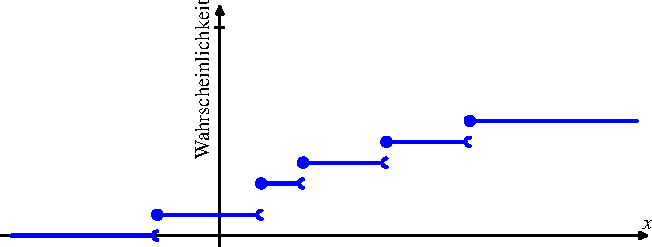
\includegraphics{images/verteilungsfunktion-3}
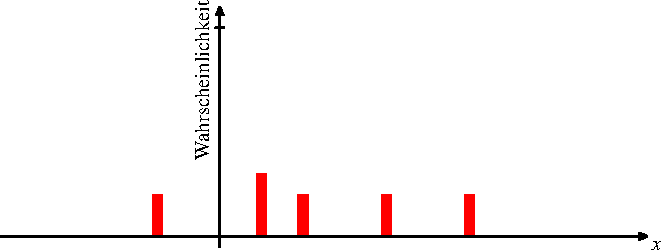
\includegraphics{images/verteilungsfunktion-5}
\end{center}
\caption{Verteilungsfunktion (oben) und Wahrscheinlichkeiten einzelner
$x$-Werte (unten) einer diskreten Verteilung
\label{bilddiskreteverteilungsfunktion}}
\end{figure}
Ist die Verteilungsfunktion st"uckweise konstant, dann ist
$P((a,b])=0$ falls im Interval $(a,b]$ keine Sprungstelle
vorhanden ist. Ist $x_0$ eine Sprungstelle, dann ist ihr H"ohe
\[
\lim_{a\to x_0-}P((a,x_0])=\lim_{a\to x_0-}(F(x_0)-F(a))
F(x_0)-\lim_{a\to x_0-}F(a).
\]
Dies bedeutet, dass $P(\{x_0\})=F(x_0)-\lim_{a\to x_0-}F(a)$.
Offensichtlich haben also nur die Sprungwerte der Funktion eine
von 0 verschiedene Wahrscheinlichkeit, alle anderen Intervalle ohne
einen Sprungpunkt haben Wahrscheinlichkeit 0. Die Wahrscheinlichkeiten
der einzelnen Sprungwerte k"onnen wie in
Abbildung~\ref{bilddiskreteverteilungsfunktion} visualisiert werden.

Ist $S=\{x|F(x)\ne \lim_{a\to x-}F(a)\}$ die Menge der Sprungpunkte 
der Verteilungsfunktion, dann kann man damit Wahrscheinlichkeiten und
Erwartungswerte wie folgt berechnen. Die Wahrscheinlichkeit eines
Ereignisses h"angt davon ab, welches Sprungpunkte es enth"alt:
\[
P(A)=\sum_{x\in S}P(\{x\}),
\]
der Erwartungswert von $f(X)$ ist
\[
E(f(X))=\sum_{x\in S}f(x)P(\{x\}).
\]
Man kann also alle relevanten Gr"ossen berechnen, wenn man f"ur jede
Sprungstelle deren Wahrscheinlichkeit weiss, also die Funktion
\[
p\colon S\to\mathbb{R}:x\mapsto p(x)=P(\{x\}).
\]
Diese Funktion muss nat"urlich den Eigenschaften einer
Wahrscheinlichkeitsfunktion Rechnung tragen, was erf"ullt ist, wenn
$p(x)\ge 0\forall x\in S$ und 
\[
\sum_{x\in S}p(x)=1.
\]
\begin{definition}Die Funktion $p\colon S\to\mathbb{R}:x\mapsto p(x)$
heisst diskrete Wahrscheinlichkeitsverteilung auf der Menge $S$.
\end{definition}
\begin{satz}F"ur eine diskrete Wahrscheinlichkeitsverteilung $p$ gilt
\begin{enumerate}
\item $\displaystyle P(A)=\sum_{x\in A\cap S}p(x)$,
\item $\displaystyle E(f(X))=\sum_{x\in S}f(x)p(x)$
\end{enumerate}
\end{satz}

\subsubsection{Stetige Verteilungsfunktion}
\begin{figure}
\begin{center}
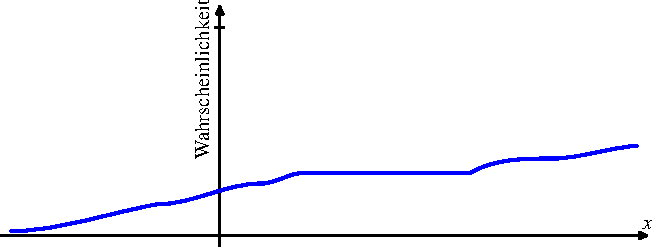
\includegraphics{images/verteilungsfunktion-4}
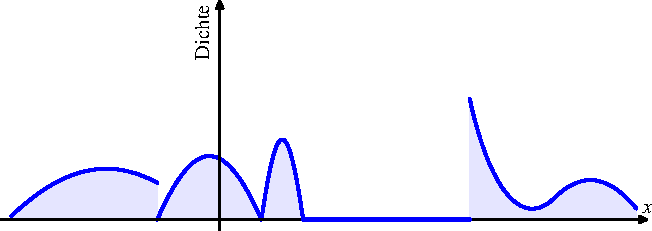
\includegraphics{images/verteilungsfunktion-6}
\end{center}
\caption{Verteilungsfunktion (oben) und Wahrscheinlichkeitsdichte 
(unten) einer stetigen Verteilung\label{bildstetigeverteilungsfunktion}}
\end{figure}
Die Formel
\[
P((a,b])=F(b)-F(a)
\]
erinnert an die Berechnung eines Integrals mit Hilfe einer
Stammfunktion.
W"are $F$ differenzierbar, k"onnte man die Ableitung bilden,
$F$ w"are dann eine Stammfunktion von $\varphi=F'$. Dann g"alte
\[
P(X\le x)=F(x)=\int_{-\infty}^x\varphi(\xi)\,d\xi.
\]
Im Allgemeinen ist selbst eine stetige Verteilungsfunktion nicht
differenzierbar.
Trotzdem gibt es dank eines Satzes, den wir hier nicht beweisen,
immer eine Funktion $\varphi$, die sich "ahnlich verh"alt wie die
Ableitung.
\begin{definition}
Die Funktion $\varphi$ heisst Wahrscheinlichkeitsdichte der Verteilungsfunktion
\index{Wahrscheinlichkeitsdichte}
\index{Dichtefunktion}
$F$ falls
\[
P(X\le x)=F(x)=\int_{-\infty}^x\varphi(\xi)\,d\xi
\]
gilt.
Man spricht in diesem Fall von einer stetigen Wahrscheinlichkeitsverteilung.
\end{definition}
Abbildung \ref{bildstetigeverteilungsfunktion} zeigt die
Wahrscheinlichkeitsdichte der stetigen Komponente der Verteilungsfunktion
aus Abbildung \ref{bildverteilungsfunktion}.

Bei diskreten Wahrscheinlichkeitsverteilungen folgte die Formel f"ur den
Erwartungswert von $X$ sofort aus der Definition, f"ur den stetigen
Fall haben wir aber noch keine exakte Definition. Wenn wir $\mathbb{R}$
in viele kleine Intervalle $I_1=(\underline x_1,\overline x_1],\dots, I_n$
unterteilen, dann gilt
\[
\sum_{i}P(I_i)\underline x_i\le
E(X)
\le
\sum_{i}P(I_i)\overline x_i
\]
Da die Wahrscheinlichkeit des Intervals $I_i$ mit Hilfe der
Wahrscheinlichkeitsdichte berechnet werden kann:
$P(I_i)=\int_{\underline x_i}^{\overline x_i}\varphi(\xi)\,d\xi,$
kann man die Ungleichung noch etwas weiter fassen:
\[
\sum_{i}\underline x_i\bigl(\min_{\xi\in I_i}\varphi(\xi)\bigr)(\overline x_i-\underline x_i)\le
E(X)
\le
\sum_{i}\overline x_i\bigl(\max_{\xi\in I_i}\varphi(\xi)\bigr)(\overline x_i-\underline x_i)
\]
L"asst man jetzt die Intervall"ange immer kleiner werden, wird wegen der
Stetigkeit von $\varphi$ der Unterschied zwischen
$\max_{\xi\in I_i}\varphi(\xi)$ und
$\min_{\xi\in I_i}\varphi(\xi)$ beliebig klein, und auch jener
zwischen $\underline x_i$ und $\overline x_i$. Beim Grenz"ubergang
zu beliebig kleinen Intervallen werden die beiden Seiten der Ungleichung
gegen das Integral
\[
\int_{-\infty}^{\infty}x\varphi(x)\,dx
\]
streben, d.h. der folgende Satz kann als Definition des Erwartungswertes
gesehen werden:
\begin{satz}
Ist $X$ eine Zufallsvariable mit stetiger
Wahrscheinlichkeitsverteilung mit Wahrscheinlichkeitsdichte
$\varphi$, dann
ist die Verteilungsfunktion $F$ "uberall dort differenzierbar, wo
$\varphi$ stetig ist, und es gilt dort
$F'(x)=\varphi(x)$.
Erwartungswerte von $X$ k"onnen mit Hilfe von
\begin{eqnarray*}
E(X)&=&\int_{-\infty}^{\infty}x\varphi(x)\,dx\quad\text{und}\\
E(f(X))&=&\int_{-\infty}^{\infty}f(x)\varphi(x)\,dx
\end{eqnarray*}
berechnet werden.
\end{satz}
\subsection{Wahrscheinlichkeit grosser Abweichungen}
Im vorhergehenden Kapitel haben wir mit dem Satz von Tschebyscheff ein
Hilfsmittel kennengelernt, welches erlaubt abzusch"atzen, dass eine
gross Abweichung vom Erwartungswert eintritt. Der Satz stellte einen
Zusammenhang mit der Varianz her:
\[
P(|X-\mu|>\varepsilon)\le\frac{\operatorname{var}(X)}{\varepsilon^2}.
\]
Es wurde damals schon bemerkt, dass f"ur ``weniger wilde'' Verteilung mit
besseren Absch"atzungen gerechnet werden kann. Insbesondere ist es mit
einer Dichtefunktion m"oglich, die Wahrscheinlichkeit einer grossen
Abweichung exakt zu berechnen:
\begin{satz} Ist $X$ eine Zufallsvariable, deren Verteilung die
Verteilungsfunktion $F$ hat, dann ist
\[
P(|X-\mu|>\varepsilon)=
1-F(\mu+\varepsilon)+\lim_{\xi\to (\mu-\varepsilon)-}F(\xi)
\]
Ist $\varphi$ eine Dichtefunktion, dann gilt
\[
P(|X-\mu|>\varepsilon)=1-\int_{\mu-\varepsilon}^{\mu+\varepsilon}\varphi(x)\,dx
\]
\end{satz}
\begin{proof}[Beweis]Die Formel f"ur die Dichtefunktion folgt offensichtlich
aus der Aussage "uber die Verteilungsfunktion, denn dann ist $F$ stetig
und der einseitige Grenzwert ist gerade der Funktionswert von $F$ an der
Stelle.
Es gen"ugt also letzteres
zu untersuchen.
\begin{eqnarray*}
P(|X-\mu|\le\varepsilon)
&=&1-P(\{X\ge\mu-\varepsilon\}\cap\{X\le\mu+\varepsilon\})\\
&=&1-F(\mu+\varepsilon)+\lim_{\xi\to (\mu-\varepsilon)-}F(\xi)
\end{eqnarray*}
\end{proof}
Eine Wahrscheinlichkeitsfunktion erlaubt also eine wesentlich
genauere Berechnung der Wahrscheinlichkeit einer grossen Abweichung,
nicht mehr nur eine grobe Absch"atzung.

\section{Beispiel: Gleichverteilung}
\index{Gleichverteilung}
Als Beispiel und zur Gegen"uberstellung stetiger und diskreter Zufallsvariablen
behandeln wir in diesem Abschnitt die diskrete und und die stetige
Gleichverteilung. Weitere Informationen zur Gleichverteilung sind
Im Abschnitt~\ref{section-gleichverteilung-stetig} zu finden.

\subsection{Ganzzahlige Gleichverteilung}
\index{Gleichverteilung!ganzzahlig}
Eine Zufallsvariable $X$ nehme die ganzzahligen Werte $\{a,a+1,\dots,b\}$ mit 
gleicher Wahrscheinlichkeit $\frac1{b-a+1}$ an.  Die Verteilungsfunktion
ist also
\[
F(x)=
\frac{\lfloor x \rfloor -a+1}{b-a+1}
\]
wobei $\lfloor x \rfloor$ die gr"osste ganze Zahl kleiner als $x$
bezeichnet:
\[
\lfloor x\rfloor = \max\{k\in\mathbb Z|k\le x\}.
\]
Die Wahrscheinlichkeitsverteilung ist
\[
P(X=x)=\begin{cases}
\frac1{b-a+1}&\qquad a\le x\le b,x\in\mathbb Z\\
0&\qquad\text{sonst}.
\end{cases}
\]
Damit kann jetzt auch Erwartungswert und Varianz bestimmt werden.
\begin{align*}
E(X)
&=
\sum_{k=a}^b kP(X=k)
=
\sum_{k=a}^b \frac{k}{b-a+1}
=
\frac1{b-a+1}\sum_{k=a}^bk^2
\\
&=
\frac1{b-a+1}\biggl(
\sum_{k=1}^bk-\sum_{k=1}^{a-1}k
\biggr)
=
\frac1{b-a+1}\biggl(
\frac{b(b+1)}2-\frac{a(a-1)}2
\biggr)
\\
&=
\frac12\frac{b^2+b-a^2+a}{b-a+1}=\frac{a+b}2.
\\
E(X^2)
&=
\sum_{k=a}^b k^2P(X=k)
=
\sum_{k=a}^b \frac{k^2}{b-a+1}
=
\frac1{b-a+1}\sum_{k=a}^bk^2
\\
&=
\frac1{b-a+1}\biggl(
\sum_{k=1}^bk^2-\sum_{k=1}^{a-1}k^2
\biggr)
=
\frac{ 2(a^2+ab+b^2)+b-a}{6}
\\
\operatorname{var}(X)
&=
\frac{ 2(a^2+ab+b^2)+b-a}{6}
-
\frac{a^2+2ab+b^2}{4}
\\
&=
\frac1{12}\bigl(
4a^2+4ab+4b^2+2b-2a-3a^2-6ab-3b^2
\bigr)
\\
&=
\frac1{12}\bigl(
a^2-2ab+b^2+2b-2a+1-1
\bigr)
=
\frac1{12}\bigl((b-a+1)^2 - 1\bigr)
\end{align*}
Die Varianz ist also im Wesentlichen die quadrierte Intervall"ange
geteilt durch 12.

\subsection{Stetige Gleichverteilung}
\index{Gleichverteilung!stetig}
\index{Gleichverteilung!auf einem Interval}
Eine Zufallsvariable $X$ nehme die Werte im Interval $[a,b]$
mit gleicher Wahrscheinlichkeit an, d.~h.~f"ur jedes Teilinterval
$[\xi,\eta]\subset[a,b]$ gilt 
\[
P(\xi\le X\le \eta)=\frac{\xi-\eta}{b-a}.
\]
Die Wahrscheinlichkeitsdichte ist dann
\[
\varphi(x)=\begin{cases}
\frac1{b-a}&\qquad a\le x\le b\\
0&\qquad \text{sonst}
\end{cases}
\]
Erwartungswert und Varianz k"onnen damit direkt berechnet werden:
\begin{align*}
E(X)
&=
\int_{-\infty}^\infty x\varphi(x)\,dx
=
\int_a^bx\frac1{b-a}\,dx
=
\frac1{b-a}\left[\frac12x^2\right]_a^b
=
\frac12\frac{b^2-a^2}{b-a}
\\
&=
\frac{a+b}2
\\
E(X^2)
&=
\int_{-\infty}^{\infty}x^2\varphi(x)\,dx
=
\int_a^bx\frac1{b-a}\,dx
=
\frac1{b-a}\left[\frac13x^3\right]_a^b
=
\frac13\frac{b^3-a^3}{b-a}
\\
&=
\frac13(b^2+ab+a^2)
\\
\operatorname{var}(X)
&=
\frac13(b^2+ab+a^2)
-
\frac14(a^2+2ab+b^2)
\\
&=
\frac1{12}(4b^2+4ab+4a^2-3a^2-6ab-3b^2
=
\frac1{12}(a^2-2ab+b^2)
\\
&=
\frac{(b-a)^2}{12}.
\end{align*}
Auch in diesem Fall ist die Varianz die quadrierte Intervall"ange
geteilt durch 12.

\section{L"osungsstrategie}
Probleme "uber Zufallsvariablen k"onnen also mit folgender L"osungsstrategie
angegangen werden.
\begin{enumerate}
\item
Zun"achst muss festgestellt werden, welche Verteilung die Zufallsvariablen
haben. Zu jeder sp"ater zu besprechenden Verteilung ist also auch
festzuhalten, f"ur welchen Zweck sie geeignet ist.
\item 
Die Verteilungen haben Parameter, die als n"achstes bestimmt werden
m"ussen.
Dazu k"onnen die bekannten Formeln f"ur Kennzahlen einer
Verteilung wie Erwartungswert oder Varianz.
So k"onnen zum Beispiel aus Erwartungswert $\mu$ und Varianz $\sigma^2$ 
einer auf einem Intervall gleichverteilten Zufallsvariable  die
Gleichungen
\begin{align*}
a+b&=2\mu\\
b^2-a^2&=12\sigma^2\quad\Rightarrow\quad b-a=\frac{6\sigma^2}{\mu}
\end{align*}
abgeleitet werden, welche $a$ und $b$ zu bestimmen erlauben. 
\item
Sobald die Parameter festliegen, k"onnen beliebige Wahrscheinlichkeiten
oder Erwartungswerte von $X$ oder Funktionen $f(X)$ ermittelt werden,
womit sich so ziemlich jede Frage beantworten l"asst.
\end{enumerate}
Im Folgenden geht es also vor allem darum, einen geeignet grossen
Katalog von Verteilungen bereitzustellen. Dazu dienen neben einigen
Grundverteilungen auch Rechenregeln, welche aus bereits bekannten
Verteilungen neue Verteilungen abzuleiten gestatten. Diese Rechenregeln
sind der Inhalt des n"achsten Abschnittes. Im folgenden Kapitel wird
dann eine Auswahl von praktisch n"utzlichen Verteilungen mit ihren
Eigenschaften vorgestellt.

\section{Rechenregeln}
Beim "Ubergang vom Wahrscheinlichkeitsraum $(\Omega,{\cal A},P)$ mit
der Zufallsvariable $X$ zur Verteilungsfunktion $F$ 
ging jede Information
"uber den Zufallsmechanismus verloren, der im Hintergrund f"ur das zuf"allige
Auftreten der verschiedenen Werte von $X$ verantwortlich war. Insbesondere
ist es bei zwei Zufallsvariablen $X$ und $Y$ nicht mehr m"oglich zu
rekonstruieren, ob sie unabh"angig oder wie gegebenenfalls die Abh"angigkeit
genau ausgesehen hat. Ohne Kenntnis von $\Omega$ ist es daher im allgemeinen
nicht mehr m"oglich, Erwartungswerte von beliebigen Funktionen von $X$ und $Y$
zu berechnen. Insbesondere $E(XY)$ l"asst sich nur berechnen, wenn man weiss,
dass $X$ und $Y$ unabh"angig sind.

Es zeigt sich also in einigen interessanten F"allen durchaus m"oglich, nur mit
Hilfe der Wahrscheinlichkeitsdichte f"ur unabh"angige
Zufallsvariable interessante Erwartungswerte zu berechnen.

\subsection{Variablentransformation}
\index{Variablentransformation}
Wendet man auf die Werte einer Zufallsvariablen eine Funktion an, entsteht
eine neue Zufallsvariable, die im Allgemeinen eine g"anzlich andere Verteilung
haben wird. In diesem Abschnitt soll die Verteilungsfunktion und falls
eine Dichte exitiert auch diese der neuen Zufallsvariablen bestimmt werden.

\index{Abbildung!umkehrbare}
Sei $f$ eine umkehrbare, differenzierbare Abbildung
$f\colon\mathbb{R}\to\mathbb{R}$. Dann ist $Y=f\circ X$ ebenfalls eine
Zufallsvariable. Bezeichnen wir die Verteilungsfunktionen von $X$ und $Y$
mit $F_X$ bzw.~$F_Y$, dann gilt offensichlich
\[
F_Y(y)=P(f\circ X\le y)=P(X\le f^{-1}(y))=F_X(f^{-1}(y))
\]
oder k"urzer $F_Y=F_X\circ f^{-1}$.

Wir nehmen nun an, dass die Verteilungsfunktionen ausserdem eine
Dichtefunktion haben, welche wir mit $\varphi_X$ bzw.~$\varphi_Y$
bezeichnen. Wir schreiben $y=f(x)$, und versuchen die obigen
Wahrscheinlichkeiten mit den Dichtefunktionen zu berechnen:
\[
P(a<Y\le b)
=\int_a^b\varphi_Y(y)\,dy
=\int_{f^{-1}(a)}^{f^{-1}(b)}\varphi_Y(f(x)) f'(x)\,dx
\]
Also muss $\varphi_Y(f(x))f'(x)$ die Wahrscheinlichkeitsdichte von
$F_X$ sein, also 
\begin{eqnarray*}
\varphi_Y(y)&=&\frac{\varphi_X(f^{-1}(y))}{f'(f^{-1}(y))}\\
\varphi_Y(f(x))&=&\frac{\varphi_X(x)}{f'(x)}
\end{eqnarray*}
Wir fassen diese Resultate in einem Satz zusammen

\begin{satz}
\label{satz-variablentransformation}
Ist $f\colon\mathbb{R}\to\mathbb{R}$ eine invertierbare
differenzierbare Funktion, deren Ableitung nirgends verschwindet,
und $X$ eine Zufallsvariable mit Verteilungsfunkion $F_X$. Dann ist
$f\circ X$ eine Zufallsvariable mit Verteilungsfunktion
$F_Y=F_X\circ f^{-1}$. Hat $F_X$ die Dichtefunktion $\varphi_X$, dann
hat $F_Y$ die Dichtefunktion
\[
\varphi_Y=\frac{\varphi_X}{f'}\circ f^{-1}.
\]
\end{satz}

Ohne zus"atzliche Annahmen ist es nicht m"oglich, Erwartungswert und
Varianz zu berechnen. Hingegen gibt es eine Gr"osse, die sich in jedem
Fall bestimmen l"asst:
\begin{definition}
Ist $X$ eine Zufallsvariable, dann heisst die Zahl $\operatorname{med}(X)$,
f"ur die
$F(\operatorname{med}(X))=\frac12$ ist, der Median von $X$. 
Falls mehrer Zahlen diese Bedingung erf"ullen, ist der Median als
deren Infimum definiert:
\[
\operatorname{med}(X)=\inf \{x\in\mathbb{R}\;|\;F(x)\ge{\textstyle \frac12}\}
\]
\end{definition}
F"ur den Median gilt $\operatorname{med}(Y)=f(\operatorname{med}(X))$.

\subsection{Standardisierung}
\index{Standardisierung}
Ein wichtiger Spezialfall ist der folgende:
aus einer Zufallsvariable $X$ mit Erwartungswert
$\mu$ und Varianz $\sigma^2$ l"asst sich eine neue Zufallsvariable $Y$ mit
Erwartungswert $0$ und Varianz $1$ konstruieren, indem man setzt
\[
Y=\frac{X-\mu}{\sigma}.
\]
Dies ist eine Variablentransformation mit der Funktion
$y=f(x)=\frac1\sigma(x-\mu)$ und der Umkehrfunktion $f^{-1}(y)=\sigma y+\mu$.
In diesem Fall kann man den Erwartungswert von $Y$ mit Hilfe der Rechenregeln
ausrechnen
\[
E(Y)=\frac1{\sigma}(E(X)-\mu)=0,
\]
und ebenso die Varianz
\[
\operatorname{var}(Y)=\frac1{\sigma^2}\operatorname{var}(X)=1.
\]
Der Satz \ref{satz-variablentransformation} l"asst sich hier unmittelbar
anwenden, es ergeben sich Verteilungs- und Dichtefunktion von $Y$
wie folgt:
\begin{eqnarray*}
F_Y(y)&=&F_X(y\sigma+\mu)\\
\varphi_Y(y)&=&\sigma\varphi_X(y\sigma+\mu)
\end{eqnarray*}
Wir fassen diese Resultate in einem Satz zusammen:

\begin{satz}
\label{satz-standardisierung}
Ist $X$ eine Zufallsvariable mit Erwartungswert $\mu$ und
Varianz $\sigma^2$, dann ist
\[
Y=\frac{X-\mu}\sigma
\]
eine Zufallsvariable mit Erwartungswert 0 und Varianz 1.
Zwischen den Verteilungsfunktionen $F_X$ bzw.~$F_Y$ von $X$ bzw.~$Y$ 
bestehen die Beziehungen
\[
F_Y(y)=F_X(y\sigma+\mu)\qquad F_X(x)=F_Y\left(\frac{x-\mu}\sigma\right)
\]
Hat die Verteilungsfunktion eine Dichte, dann gilt ausserdem
\[
\varphi_Y(y)=\sigma\varphi_X(y\sigma+\mu)\qquad
\varphi_X(x)=\frac1{\sigma}\varphi_Y\left(\frac{x-\mu}\sigma\right)
\]
\end{satz}


\subsection{Zwei Zufallsvariable}
Wir beschr"anken uns darauf, die Wahrscheinlichkeitsdichten von Summen
und Produkten von Zufallsvariablen zu berechnen, die wir als unabh"angig
voraussetzen.
Wir betrachten also zwei Zufallsvariable $X_1$ und $X_2$ mit reellen
Werten.
Da die Werte voneinander unabh"angig sind, ist
die passende Ereignisalgebra die Produktalgebra, also
$(x_1,x_2)\in
\mathbb{R}\times\mathbb{R}$,
und die Ereignisse sind kartesiches Produkte von Intervallen. Dann sind
die Wahrscheinlichkeiten $P(X_1\le x_1)$  und $P(X_2\le x_2)$ unabh"angig
voneinander, insbesondere ist $P(X_1\le x_1)=F_1(x_1)$ und
$P(X_2\le x_2)=F_2(x_2)$.

Die Wahrscheinlichkeit, dass $X_1$ in einem Intervall $(a_1,b_1]$,
$X_2$ im Interval $(a_2,b_2]$ liegt ist 
\begin{eqnarray*}
P(a_1<X_1\le b_1\wedge a_2<X_2\le b_2)
&=& P(a_1<X_1\le b_1) P(a_2<X_2\le b_2)\\
&=&\int_{a_1}^{b_1}\varphi_1(x_1)\,dx_1
\int_{a_2}^{b_2}\varphi_2(x_2)\,dx_2\\
&=&\int_{a_1}^{b_1}dx_1
\int_{a_2}^{b_2}dx_2\,
\varphi_1(x_1) \varphi_2(x_2).
\end{eqnarray*}
Die zweidmensionale
Verteilungsfunktion $F(x_1,x_2)=P(X_1\le x_1\wedge X_2\le x_2)$ hat
also eine zweidimensionale Wahrscheinlichkeitsdichte
\[
\varphi(x_1,x_2)=\varphi_1(x_1)\varphi_2(x_2).
\]

\subsection{Summe zweier Zufallsvariable}
\index{Summe zweier Zufallsvariablen}
Seien $X_1$ und $X_2$ zwei Zufallsvariable mit Verteilungsfunktion $F_1$ und
$F_2$. Gesucht ist die Verteilungsfunktion $F$ von $X_1+X_2$, sowie die
Wahrscheinlichkeitsverteilung und gegebenenfalls die Wahrscheinlichkeitsdichte.

Zun"achst ist nach Definition der Verteilungsfunktion
\[
F(z)=P(X_1+X_2\le z).
\]
Die Berechnung von $F$ aus $F_1$ und $F_2$ verl"auft f"ur diskrete und
kontinuierliche Wahrscheinlichkeitsverteilungen verschieden.
\subsubsection{Diskreter Fall}
In diesem Fall hat $X_i$ die Wahrscheinlichkeitsverteilung
$p_i(x)$ auf der Menge $S_i$, und es gilt
\begin{eqnarray*}
F(z)&=&\sum_{x_1\in S_1, x_2\in S_2, x_1+x_2\le z}p(x_1)p(x_2)\\
&=&\sum_{x_1\in S_1}p(x_1)\sum_{x_2\in S_2, x_2 \le z - x_1}p(x_2)\\
&=&\sum_{x_1\in S_1}p(x_1) F_2(z-x_1)
\end{eqnarray*}
Oder, wenn vor allem die Wahrscheinlichkeitsverteilung interessiert:
\[
p(z)=\sum_{x_1\in S_1, x_2\in S_2, x_1+x_1=z}p(x_1)p(x_2).
\]
\subsubsection{Stetiger Fall}
Im stetigen Fall kann man schreiben
\begin{eqnarray*}
F(z)&=&\int_{-\infty}^{\infty}\int_{-\infty}^{z-x_1}\varphi_1(x_1)\varphi_2(x_2)
\,dx_2\,dx_1\\
&=&\int_{-\infty}^{\infty}
\varphi_1(x_1)
\int_{-\infty}^{z-x_1}
\varphi_2(x_2)
\,dx_2\,dx_1\\
&=&\int_{-\infty}^{\infty}
\varphi_1(x_1)
F_2(z-x_1)
\,dx_1\\
\end{eqnarray*}
Nun interesssiert uns vor allem die Wahrscheinlichkeitsdichte, also die
``Ableitung'' von $F$:
\[
\varphi(z)=\int_{-\infty}^{\infty}\varphi_1(x_1)\varphi_2(z-x_1)\,dx_1
\]
Diese Integral heisst die Faltung der Funktionen $\varphi_1$ und $\varphi_2$,
$\varphi=\varphi_1*\varphi_2$.
\index{Faltung}

\subsection{Verteilung von $X^2$}
Wir bestimmen die Wahrscheinlichkeitsdichte f"ur das Quadrat 
$X^2$ einer stetig verteilte Zufallsvariable $X$.
Sei $F_{X^2}$ die Verteilungsfunktion von $X^2$, $F_X$ jene von $X$.
Dann gilt f"ur $z\ge 0$
\begin{eqnarray*}
F_{X^2}(z)&=&P(X^2\le z)=P(-\sqrt{z}\le X\le \sqrt{z})\\
&=&F_X(\sqrt{z})-F(-\sqrt{z})\\
&=&\int_{-\infty}^{\sqrt{z}}\varphi(x)\,dx-\int_{-\infty}^{-\sqrt{z}}\varphi(x)\,dx\\
&=&\int_{-\sqrt{z}}^{\sqrt{z}}\varphi(x)\,dx
\end{eqnarray*}
F"ur negative $z$ verschwindet die Verteilungsfunktion nat"urlich, denn
die Wahrscheinlichkeit dass $X^2\le z <0$ ist nat"urlich 0.

Wir interessieren uns aber wieder nur f"ur Dichtefunktion, die wir
durch Ableiten finden k"onnen:
\[
\varphi_{X^2}(z)=\begin{cases}
\frac{1}{2\sqrt{z}}\left(\varphi_X(\sqrt{z})+\varphi_X(-\sqrt{z})\right)&\qquad z\ge 0\\
0&\qquad z<0
\end{cases}
\]
Weitere Beispiele f"ur aus mehreren unabh"angigen Zufallsvariablen
verkn"upften Verteilungen werden wir weiter unten behandeln, wobei
dann auch eine konkrete Wahrscheinlichkeitsdichtefunktion gegeben sein
wird.

\subsection{Verteilung von $\sqrt{X}$\label{verteilungsfunktion-wurzel}}
Sei $X$ eine Zufallsvariable mit $X\ge 0$. Hat $X$ Verteilungsfunktion $F_X$
und Dichtefunktion
$\varphi_X$, dann ist die Verteilungsfunktion von $\sqrt{X}$
\[
F_{\sqrt{X}}(x)=P(\sqrt{X}\le x)=P(X\le x^2)=F_X(x^2)
\]
F"ur die Dichtefunktionen bedeutet das
\[
F_{\sqrt{X}}(x)=\int_0^{x^2}\varphi_X(t)\,dt
\]
woraus man die Dichtefunktion $\varphi_{\sqrt{X}}$ durch ableiten
bestimmen kann:
\[
\varphi_{\sqrt{X}}(x)=2x\varphi_X(x^2).
\]

\subsection{Verteilung von $X/Y$\label{verteilungsfunktion-quotient}}
Seien $X$ und $Y$ Zufallsvariablen mit $Y>0$, dann ist $T=X/Y$ ebenfalls
eine Zufallsvariable. Ist $\varphi_Y$ die Dichtefunktion von $Y$,
und $F_X$ die Verteilungsfunktion von $X$, dann kann man die
Verteilungsfunktion von $T$ wie folgt berechnen:
\[
P(T\le t)=P(X\le tY)=\int_0^\infty F_X(ty)\varphi_Y(y)\,dy
\]
Die Ableitung nach $t$ ergibt die zugeh"orige Dichtefunktion
\[
\varphi_T(t)=\int_0^\infty\varphi_X(ty)y\varphi_Y(y)\,dy.
\]

\subsection{Verteilung von $XY$\label{verteilungsfunktion-produkt}}
\index{Produkt zweier Zufallsvariable}
Seien $X$ und $Y$ unabh"angige, positive Zufallsvariable, dann ist $T=XY$
ebenfalls eine Zufallsvariable. Wir suchen die Warhscheinlichkeitsdichte
$\varphi_T$ von $T$.  Zun"achst gilt nach Definition
\[
F_T(t)=P(XY\le t).
\]
Die Wahrscheinlichkeit, dass $X$ einen Wert in einem sehr schmalen Interval
$[x,x+dx]$ annimmt ist $\varphi_X(x)\,dx$.
Damit beim Eintreffen dieses Ereignisses auch das Produkt
$XY\le t$ ist, muss $Y$ einen Wert im Interval $[0,t/x]$ annehmen.
Also gilt wegen der Unabh"angigkeit von $X$ und $Y$
\begin{eqnarray*}
P(XY\le t\;\wedge\; X\in[x,x+dx])&=&P(X\in[x,x+dx]\;\wedge\; Y\le t/x)\\
&=&P(X\in[x,x+dx])\cdot P(Y\le t/x)\\
&=&\varphi_X(x)\,dx\cdot F_Y(t/x).
\end{eqnarray*}
Um nun die gesamte Wahrscheinlichkeit $P(XY\le t)$ zu finden, m"ussen die eben
berechneten Terme ``summiert'' werden:
\[
P(XY\le t)=\int_0^\infty\varphi_X(x)F_Y(t/x)\,dx
\]
Durch Ableiten nach $t$ findet man
\[
\varphi_{XY}(t)=\frac{d}{dt}F_{XY}(t)=\int_0^\infty \varphi_X(x)\varphi_Y(t/x)\,\frac{dx}x.
\]



